\section{Multi-dimensional problems}

We can now generalize the concepts from one-dimensional spatial domains to the more realistic multi-dimensional case.


\subsection{General form}

Systems of hyperbolic conservation laws in multiple space dimensions \(x \in \Omega \subset \R^d\) for the unknown \(U: \Omega \times \R^+ \to \R^N\) have the form
\[
	\partial_t U + \partial_{x_1}F^{\parentheses*{1}}\parentheses*{U} + \cdots + \partial_{x_d}F^{\parentheses*{d}}\parentheses*{U} = 0,
\]
with flux functions \(F^{\parentheses*{i}}: \R^N \to \R^N, i = 1, \ldots, d\).
Alternatively, we can simply write this as
\[
	\partial_t U + \div\mathcal{F}\parentheses*{U} = 0,
\]
with matrix-valued flux
\[
	\mathcal{F}: \R^N \to \R^{N \times d}, U \mapsto \mathcal{F}\parentheses*{U} = \parentheses*{F^{\parentheses*{1}}\parentheses*{U}, \ldots, F^{\parentheses*{d}}\parentheses*{U}},
\]
where the divergence acts on the columns.

\begin{example}[Multi-dimensional equations]
	 \begin{enumerate}
	 	\item Consider a \emph{\(2\)-dimensional advection} in the direction \(\parentheses*{a, b} \in \R^2\).
	 	The unknown is \(u: \R^2 \times \R^+ \to \R\) and the corresponding conservation law reads
	 	\[
	 		\partial_t u + a\partial_x u + b\partial_y u = 0, \quad \parentheses*{x, y} \in \R^2, t > 0, \quad u\parentheses*{x, y, 0} = u_0\parentheses*{x, y}.
	 	\]
	 	The exact solution is given again by dimension-wise translation/transport:
	 	\[
	 		u\parentheses*{x, y, t} = u_0\parentheses*{x - at, y - bt}.
	 	\]
	 	\item Consider now the \emph{\(2\)-dimensional Euler equations of gas dynamics} with unknown solution vector
	 	\[
	 		U = \parentheses*{\rho, \rho v_x, \rho v_y, E_{\text{tot}}},
	 	\]
	 	with density \(\rho\), velocity \(\parentheses*{v_x, v_y} \in \R^2\), and \emph{total energy}
	 	\[
	 		E_{\text{tot}} = \frac{1}{\gamma - 1}p + \frac{1}{2}\rho\parentheses*{v_x^2 + v_y^2}
	 	\]
	 	with pressure \(p\).
	 	The flux functions in \(x\)- and \(y\)-direction are
	 	\[
	 		F^{\parentheses*{x}}\parentheses*{U} = F\parentheses*{U} = \begin{pmatrix}
	 			\rho v_x\\
	 			\rho v_x^2 + p\\
	 			\rho v_x v_y\\
	 			\parentheses*{E_{\text{tot}} + p}v_x
	 		\end{pmatrix}, \quad F^{\parentheses*{y}}\parentheses*{U} = G\parentheses*{U} = \begin{pmatrix}
	 			\rho v_x\\
	 			\rho v_x v_y\\
	 			\rho v_y^2 + p\\
	 			\parentheses*{E_{\text{tot}} + p}v_y
	 		\end{pmatrix}.
	 	\]
	 \end{enumerate}
\end{example}


\subsection{Splitting methods}

A convenient approach to handle these multidimensional conservation laws is by considering each partial derivative as a separate operator.
This then allows to take advantage of the general concept of operator splitting, which we describe next.
Specifically, we consider a very general form of a partial differential equation
\[
	\partial_t u = \mathcal{A}\parentheses*{u} + \mathcal{B}\parentheses*{u},
\]
with ``evolution operators'' \(\mathcal{A}\) and \(\mathcal{B}\).

\begin{example}
	Practically all realistic applications have multiple operators.
	For example:
	\begin{enumerate}
		\item multi-dimensional conservation laws, for example for \(d = 2\)
		\[
			\partial_t U + \partial_x F\parentheses*{U} + \partial_y G\parentheses*{U} = 0,
		\]
		where the operators are
		\[
			\mathcal{A}\parentheses*{u} = -\partial_x F\parentheses*{u}, \quad \mathcal{B}\parentheses*{u} = -\partial_y G\parentheses*{u}.
		\]
		\item \emph{relaxational balance laws} with some algebraic right-hand side \(P\parentheses*{U}\)
		\[
			\partial_t U + \partial_x F\parentheses*{U} = P\parentheses*{U},
		\]
		where the operators are
		\[
			\mathcal{A}\parentheses*{u} = -\partial_x F\parentheses*{u}, \quad \mathcal{B}\parentheses*{u} = P\parentheses*{u}.
		\]
		The simplest example for this case is an advection equation with decay
		\[
			\partial_t u + a\partial_x u = -\beta u.
		\]
		When equipped with an initial condition \(u_0: \R \to \R\), the exact solution is
		\[
			u\parentheses*{x, t} = u_0\parentheses*{x - at}e^{-\beta t}.
		\]
	\end{enumerate}
\end{example}

\begin{theorem}[Splitting methods]
	Let \(\mathcal{A}\) and \(\mathcal{B}\) be linear operators.
	A splitting method considers the two evolution equations
	\begin{equation}\label{eq:15-1}
		\partial_t v = \mathcal{A}\parentheses*{v}
	\end{equation}
	and
	\begin{equation}\label{eq:15-2}
		\partial_t v = \mathcal{B}\parentheses*{v}
	\end{equation}
	separately.
	Let \(u\parentheses*{t}\) be the solution at time \(t\) of the full equation \(\partial_t u = \mathcal{A}\parentheses*{u} + \mathcal{B}\parentheses*{u}\).
	Then the following two splitting variants are common:
	\begin{enumerate}
		\item \emph{Gudunov splitting}: \(u\parentheses*{t} \xrightarrow{\eqref{eq:15-1}\text{ with }\Delta t}u^*\parentheses*{t} \xrightarrow{\eqref{eq:15-2}\text{ with }\Delta t} \tilde{u}\parentheses*{t + \Delta t}\).

		The local error satisfies
		\[
			\norm*{u\parentheses*{t + \Delta t} - \tilde{u}\parentheses*{t + \Delta t}} = \mathcal{O}\parentheses*{\Delta t^2}.
		\]
		\item \emph{Strang splitting}: \(u\parentheses*{t} \xrightarrow{\eqref{eq:15-1}\text{ with }\frac{\Delta t}{2}}u^*\parentheses*{t} \xrightarrow{\eqref{eq:15-2}\text{ with }\Delta t} u^{**}\parentheses*{t} \xrightarrow{\eqref{eq:15-1}\text{ with }\frac{\Delta t}{2}} \tilde{u}\parentheses*{t + \Delta t}\).

		The local error satisfies
		\[
			\norm*{u\parentheses*{t + \Delta t} - \tilde{u}\parentheses*{t + \Delta t}} = \mathcal{O}\parentheses*{\Delta t^3}.
		\]
	\end{enumerate}
\end{theorem}

\begin{proof}
	Consider a Taylor expansion of the exact solution to the full equation
	\[
		u\parentheses*{t + \Delta t} = u\parentheses*{t} + \Delta t\partial_t u + \frac{\Delta t^2}{2}\partial_{tt}u + \cdots = \sum_{p = 0}^\infty \frac{\Delta t^p}{p!}\partial_t^p u\parentheses*{t}.
	\]
	As \(\mathcal{A}\) and \(\mathcal{B}\) are linear operators we have \(\partial_t u = \parentheses*{\mathcal{A} + \mathcal{B}}u\) and \(\partial_t^p u = \parentheses*{\mathcal{A} + \mathcal{B}}^p u\), and thus
	\[
		u\parentheses*{t + \Delta t} = \sum_{p = 0}^\infty \frac{\Delta t^p}{p!}\parentheses*{\mathcal{A} + \mathcal{B}}^p u\parentheses*{t}.
	\]
	For the soluitons \(\hat{u}\) and \(\hat{\hat{u}}\) to sub-problems \eqref{eq:15-1} and \eqref{eq:15-2}, respectively, we find
	\[
		\hat{u}\parentheses*{t + \Delta t} = \sum_{p = 0}^\infty \frac{\Delta t^p}{p!}\mathcal{A}^p \hat{u}\parentheses*{t} \quad \text{and} \quad \hat{\hat{u}}\parentheses*{t + \Delta t} = \sum_{p = 0}^\infty \frac{\Delta t^p}{p!}\mathcal{B}^p \hat{\hat{u}}\parentheses*{t},
	\]
	analogously.
	The Godunov splitting method (i) first maps \(u\parentheses*{t}\) via \eqref{eq:15-1} to
	\[
		u^*\parentheses*{t} = \sum_{p = 0}^\infty \frac{\Delta t^p}{p!}\mathcal{A}^p u\parentheses*{t}
	\]
	and then this via \eqref{eq:15-2} to
	\[
		\tilde{u}\parentheses*{t + \Delta t} := \sum_{q = 0}^\infty \frac{\Delta t^q}{q!}\mathcal{B}^q u^*\parentheses*{t} = \sum_{q = 0}^\infty \frac{\Delta t^q}{q!}\mathcal{B}^q \sum_{p = 0}^\infty \frac{\Delta t^p}{p!}\mathcal{A}^p u\parentheses*{t} = \sum_{q = 0}^\infty \sum_{p = 0}^\infty \frac{\Delta t^q}{q!}\frac{\Delta t^p}{p!}\mathcal{A}^p \mathcal{B}^q u\parentheses*{t}.
	\]
	Comparison with the exact solution gives
	\[
		u\parentheses*{t + \Delta t} - \tilde{u}\parentheses*{t + \Delta t} = \frac{\Delta t^2}{2}\parentheses*{\mathcal{A}\mathcal{B} - \mathcal{B}\mathcal{A}}u\parentheses*{t} + \mathcal{O}\parentheses*{\Delta t^3},
	\]
	where the factor does not vanish since the operators do not commute.
	The error for Strang splitting method (ii) follows analogously.
\end{proof}

\begin{remark}
	\begin{enumerate}
		\item Typically, the sub-problems \eqref{eq:15-1} and \eqref{eq:15-2} will not be solved exactly, but also with some numerical approximation.
		That is, the splitting method adds an additional error to the usual discretization errors.
		\item After \(n = \frac{T}{\Delta t}\) time steps the local errors add up to \(\mathcal{O}\parentheses*{\Delta t}\) for Gudonov splitting and \(\mathcal{O}\parentheses*{\Delta t^2}\) for Strang.
		\item Very often the splitting error turns out to be small.
	\end{enumerate}
\end{remark}

\begin{example}[Commuting vs. non-commuting operators]
	Consider the relaxational balance law for \(u\parentheses*{x, t}\)
	\[
		\partial_t u + a\partial_x u = -\beta\parentheses*{x}u,
	\]
	with \(a \in \R\) and the linear operators
	\[
		\mathcal{A}\parentheses*{u} = -a\partial_x u \quad \text{and} \quad \mathcal{B}\parentheses*{u} = -\beta u.
	\]
	If the function \(\beta: \R \to \R\) is constant, we can easily compute the error constant of the Godunov splitting and find
	\[
		\parentheses*{\mathcal{A}\mathcal{B} - \mathcal{B}\mathcal{A}}u = -a\partial_x \parentheses*{-\beta u} - \parentheses*{-\beta}\parentheses*{-a\partial_x u} = 0,
	\]
	so that we have no \(\mathcal{O}\parentheses*{\Delta t^2}\) splitting error and the overall local error is actually \(\mathcal{O}\parentheses*{\Delta t^3}\).
	However, for a non-constant \(\beta\parentheses*{x}\) we find
	\[
		\parentheses*{\mathcal{A}\mathcal{B} - \mathcal{B}\mathcal{A}}u = -a\partial_x \parentheses*{-\beta\parentheses*{x} u} - \parentheses*{-\beta\parentheses*{x}}\parentheses*{-a\partial_x u} = a\beta'\parentheses*{x}u \ne 0,
	\]
	hence there will be an \(\mathcal{O}\parentheses*{\Delta t^2}\) splitting error.
\end{example}


\subsection{Multi-dimensional advection}

Based on these operator splitting concepts, below we list several basic ideas to discretize the \(2\)-dimensional advection equation
\[
	\partial_t u + a\partial_x u + b\partial_y u = 0, \quad \parentheses*{x, y} \in \R^2, t > 0, \quad u\parentheses*{x, y, 0} = u_0\parentheses*{x, y},
\]
with \(a, b > 0\).
We consider a simple Cartesian grid in \(\R^2\) with grid sizes \(\Delta x\) and \(\Delta y\), grid points \(\parentheses*{x_i, y_i}\), and discretized point values
\[
	u_{i, j}^n = u\parentheses*{x_i, y_j, t_n}.
\]
Based on what we have seen for conservation laws in one spatial variable, the following approaches appear natural:
\begin{enumerate}
	\item We could use the upwind discretization for each derivative, that is, separately for each coordinate:
	\[
		u_{i, j}^{n + 1} = u_{i,j}^n + \frac{a\Delta t}{\Delta x}\parentheses*{u_{i - 1, j}^n - u_{i, j}^n} + \frac{b\Delta t}{\Delta y}\parentheses*{u_{i, j - 1}^n - u_{i, j}^n}.
	\]
	This approach is sometimes called \emph{additive splitting}.
	\item Alternatively, we can use upwind in a standard Godunov timestep splitting method (\emph{multiplicative splitting}).
	That is,
	\[
		u_{i, j}^* = u_{i, j}^n + \frac{a\Delta t}{\Delta x}\parentheses*{u_{i - 1, j}^n - u_{i, j}^n}, \quad u_{i, j}^{n + 1} = u_{i, j}^* + \frac{b\Delta t}{\Delta y}\parentheses*{u_{i, j - 1}^* - u_{i, j}^*},
	\]
	which eventually gives
	\begin{align*}
		u_{i, j}^{n + 1} = &u_{i, j} + \frac{a\Delta t}{\Delta x}\parentheses*{u_{i - 1, j}^n - u_{i, j}^n} + \frac{b\Delta t}{\Delta y}\parentheses*{u_{i, j - 1}^n - u_{i, j}^n}\\
		&+ \frac{ab\Delta t^2}{\Delta x\Delta y}\parentheses*{u_{i - 1, j - 1}^n - u_{i, j - 1}^n - u_{i - 1, j}^n + u_{i, j}^n}.
	\end{align*}
	\item Using the Lax-Wendroff approach, which is based on the solution's Taylor expansion
	\[
		u\parentheses*{x, y, t + \Delta t} = u\parentheses*{x, y, t} + \Delta t\partial_t u + \frac{1}{2}\Delta t^2 \partial_{tt}u + \mathcal{O}\parentheses*{\Delta t^3},
	\]
	we replace the time derivatives with spatial derivatives using the relations
	\[
		\partial_t u = -a\partial_x u - b\partial_y u, \quad \partial_{tt}u = -a\partial_x \parentheses*{\partial_t u} - b\partial_y \parentheses*{\partial_t u} = a^2 \partial_{xx}u + b\partial_{yy}u + 2ab\partial_{xy}u.
	\]
	Using central finite difference approximations for all derivatives we obtain
	\begin{align*}
		u_{i, j}^{n + 1} = &u_{i, j}^n + \frac{a\Delta t}{2\Delta x}\parentheses*{u_{i - 1, j}^n - u_{i + 1, j}^n} + \frac{b\Delta t}{2\Delta y}\parentheses*{u_{i, j - 1}^n - u_{i, j + 1}^n}\\
		&+ \frac{a^2 \Delta t^2}{2\Delta x^2}\parentheses*{u_{i - 1, j}^n - 2u_{i, j}^n + u_{i + 1, j}^n} + \frac{b^2 \Delta t^2}{2\Delta y^2}\parentheses*{u_{i, j - 1}^n - 2u_{i, j}^n - u_{i, j + 1}^n}\\
		&+ \frac{ab\Delta t^2}{4\Delta x\Delta y}\parentheses*{u_{i - 1, j - 1}^n - u_{i, j - 1}^n - u_{i - 1, j}^n + u_{i, j}^n}.
	\end{align*}
	This is almost like two super-imposed 1D-LW, but includes one cross derivative.
	\item Similar to the Godunov method, the \emph{corner transport} method considers the exact evolution of the piecewise constant grid function in 2D.
	\begin{center}
		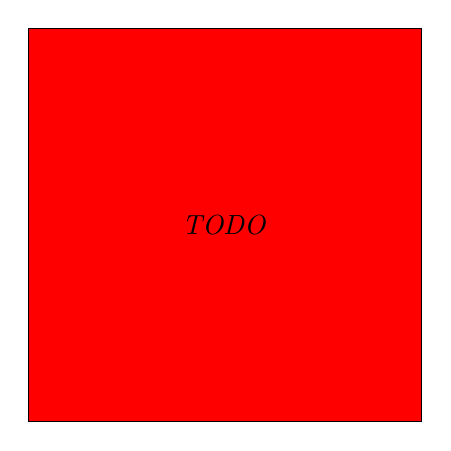
\begin{tikzpicture}
			\filldraw[fill=red] (0,0) rectangle (5,5) node[pos=.5] {\emph{TODO}};
		\end{tikzpicture}
	\end{center}
	For the advection equation, the exact solution is \(\tilde{u}\parentheses*{x, y, t_n + \Delta t} = u_{\Delta x, \Delta y}^n\parentheses*{x - a\Delta t, y - b\Delta t}\), which we integrate to obtain new cell mean values
	\begin{align*}
		u_{i, j}^{n + 1} = &\frac{1}{\Delta x\Delta y}\int_{x_{i - \frac{1}{2}}}^{x_{i + \frac{1}{2}}}\int_{y_{j - \frac{1}{2}}}^{y_{j + \frac{1}{2}}}u_{\Delta x, \Delta y}^n\parentheses*{x - a\Delta t, y - b\Delta t}\d y\d x\\
		= &u_{i, j}^n + \frac{a\Delta t}{2\Delta x}\parentheses*{u_{i - 1, j}^n - u_{i + 1, j}^n} + \frac{b\Delta t}{2\Delta y}\parentheses*{u_{i, j - 1}^n - u_{i, j + 1}^n}\\
		&+ \frac{ab\Delta t^2}{\Delta x\Delta y}\parentheses*{u_{i - 1, j - 1}^n - u_{i, j - 1}^n - u_{i - 1, j}^n + u_{i, j}^n}.
	\end{align*}
	This is the same as upwind and splitting, because the operators commute.
\end{enumerate}
We summarize basic properties of these numerical schemes below.

\begin{theorem}[Two-dimensional advection]
	For \(2\)-dimensional advection with \(a, b > 0\) the following consistency orders and linear stability conditions hold:
	\begin{enumerate}
		\item \emph{pure upwind}: order \(p = 1\), and \(0 \le \nu_x + \nu_y \le 1\),
		\item \emph{upwind splitting} and \emph{corner transport}: order \(p = 1\), and \(0 \le \max\parentheses*{\nu_x, \nu_y} \le 1\),
		\item \emph{2D Lax-Wendroff}: order \(p = 2\), and \(\nu_x^2 + \nu_y^2 \le 1\),
	\end{enumerate}
	with Courant numbers \(\nu_x + \frac{a\Delta t}{\Delta x}\) and \(\nu_y = \frac{b\Delta t}{\Delta y}\), respectively.
\end{theorem}

\begin{proof}[Idea of Proof]
	Consistency can be checked, as usual, based on Taylor expansions.
	For the stability one uses the von-Neumann approach, in 2D, that is the representation \(u_{i, j}^n = \sum_{k = 1}^N \sum_{\ell = 1}^N \hat{u}_{k, \ell}^n e^{i\parentheses*{k\pi x_i + \ell\pi y_i}}\).
\end{proof}

\begin{remark}
	\begin{enumerate}
		\item The stability conditions can be visualized in a \(\parentheses*{\nu_x, \nu_y}\)-plot.
		\begin{center}
			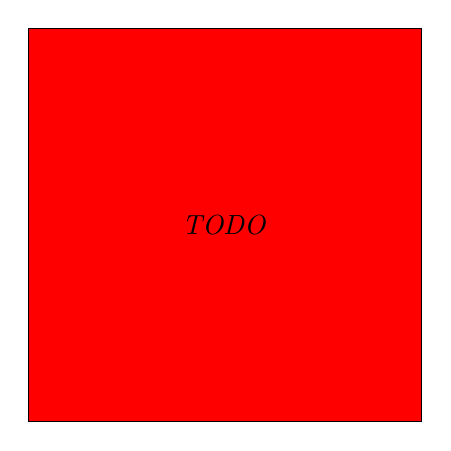
\begin{tikzpicture}
				\filldraw[fill=red] (0,0) rectangle (5,5) node[pos=.5] {\emph{TODO}};
			\end{tikzpicture}
		\end{center}
		\item The Lax-Wendroff (LW) method also allows \(a, b < 0\), but if upwinding is implemented by respecting the advection direction in 1D (see earlier sections), then upwind with Godunov splitting has the best stability condition
		\[
			\max\parentheses*{\absolute*{\nu_x}, \absolute*{\nu_y}} \le 1.
		\]
	\end{enumerate}
\end{remark}


\subsection{General FV-methods in 2D}

Let \(\mathcal{T}\) be a regular grid that covers \(\Omega \in \R^d\), based in cells or \emph{finite volumes} \(\braces*{K_i}_{i = 1, \ldots, n}\), that are triangles, quadrilaterals, or general polygons in 2D; similarly tetrahedrons, hexagons, etc. in 3D.
We consider as numerical discretization the cell mean value
\[
	\bar{U}_{K_i}\parentheses*{t} := \frac{1}{\absolute*{K_i}}\int_{K_i}U\parentheses*{x, t}\d x,
\]
using \(\absolute*{K_i}\) to denote the finite volume's ``measure'' or size (i.e., its area in 2D, its volume in 3D, etc.).
Integrating the conservation law
\[
	\partial_t U + \div\mathcal{F}\parentheses*{U} = 0
\]
over each finite volume \(K_i\) and dividing by \(\absolute*{K_i}\), we obtain the integral formulations
\[
	\frac{\d}{\d t}\bar{U}_{K_i} = -\frac{1}{\absolute*{K_i}}\int_{K_i}\div\mathcal{F}\parentheses*{U}\d x = -\frac{1}{\absolute*{K_i}}\int_{\partial K_i}\mathcal{F}\parentheses*{U}\bm{n}\d s \equiv -\frac{1}{\absolute*{K_i}}\int_{\partial K_i}F_{\bm{n}}\parentheses*{U}\d s,
\]
based on the flux through the boundary \(K_i\) with normal vector \(\bm{n} \in \R^d\).
Here \(F_{\bm{n}}: \R^N \to \R^N\) denotes the \emph{quasi-1D flux function} given by
\[
	F_{\bm{n}}\parentheses*{U} := \mathcal{F}\parentheses*{U}\bm{n} = \sum_{j = 1}^d n_j F^{\parentheses*{j}}\parentheses*{U}.
\]
In particular, for two spatial dimensions (i.e., \(d = 2\)) it is common to approximate the flux integral by a sum over the cell edges using a midpoint quadrature
\[
	\frac{1}{\absolute*{K_i}}\int_{\partial K_i}F_{\bm{n}}\parentheses*{U}\d s \approx \frac{1}{\absolute*{K_i}}\sum_{j\text{ edges}}\norm*{\bm{e}_j}\left.F_{\bm{n}_j}\parentheses*{U}\right|_{\text{midpoint of }\bm{e}_j},
\]
where \(\bm{n}_j\) is the normal edge \(\bm{e}_j\) of the finite volume \(K_i\).
\begin{center}
	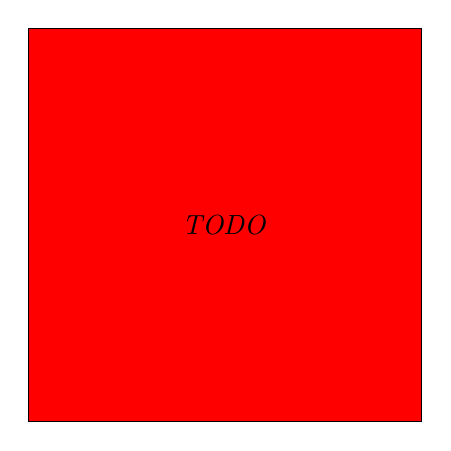
\begin{tikzpicture}
		\filldraw[fill=red] (0,0) rectangle (5,5) node[pos=.5] {\emph{TODO}};
	\end{tikzpicture}
\end{center}

\begin{definition}[Semi-discrete, two-dimensional FVM]
	For the time-dependent cell mean values \(\bar{U}_{K_i}\parentheses*{t}\) on cells \(\braces*{K_i}_{i = 1, \ldots, N}\), the \emph{first order semi-discretization} of a system of conservation laws is given by
	\[
		\frac{\d}{\d t}\bar{U}_{K_i}\parentheses*{t} = -\sum_{j\text{ edges}}\frac{\norm*{\bm{e}_j}}{\absolute*{K_i}}\tilde{F}_{\bm{n}_j}\parentheses*{\bar{U}_{K_i}\parentheses*{t}, \bar{U}_{\tilde{K}^{\parentheses*{j}}}\parentheses*{t}},
	\]
	which is based on a consistent numerical flux \(\tilde{F}_{\bm{n}_j}\) for the projected, quasi-1D flux \(F_{\bm{n}_j}\) in the direction of \(\bm{n}_j\) for each edge \(\bm{e}_j\) of cell \(K_i\).
	Moreover, the consistent numerical flux depends on the cell mean value of cell \(K_i\) and on the cell mean value of the neighboring cell \(\tilde{K}^{\parentheses*{j}}\) across the edge \(\bm{e}_j\).
\end{definition}

\begin{remark}
	\begin{enumerate}
		\item The numerical flux function is constructed essentially as for a one-dimensional Riemann problem consisting of the two adjacent cell mean values.
		\begin{center}
			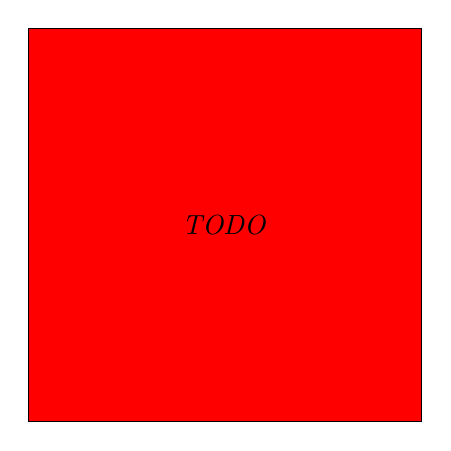
\begin{tikzpicture}
				\filldraw[fill=red] (0,0) rectangle (5,5) node[pos=.5] {\emph{TODO}};
			\end{tikzpicture}
		\end{center}
		\item To increase the spatial accuracy the solution in each cell can be reconstructed, for example, as a linear function using the neighboring values.
		A multi-dimensional generalization of the min-mod limiter would, for example, select the reconstruction with the smallest absolute slope.
	\end{enumerate}
\end{remark}

\begin{example}[Cartesian FV in 2D]
	Consider the uniform rectangles with cell center at \(\parentheses*{x_i, y_i}\) size \(\Delta x \times \Delta y\).
	Obviously, \(\absolute*{K} = \Delta x\Delta y\) and each cell as four edges
	\[
		\bm{e}_1 = \begin{pmatrix}
			0\\
			\Delta y
		\end{pmatrix}, \quad \bm{e}_2 = \begin{pmatrix}
			-\Delta x\\
			0
		\end{pmatrix}, \quad \bm{e}_3 = \begin{pmatrix}
			0\\
			-\Delta y
		\end{pmatrix}, \quad \bm{e}_4 = \begin{pmatrix}
			\Delta x\\
			0
		\end{pmatrix}
	\]
	with corresponding normal vectors
	\[
		\bm{n}_1 = \begin{pmatrix}
			1\\
			0
		\end{pmatrix}, \quad \bm{n}_2 = \begin{pmatrix}
			0\\
			1
		\end{pmatrix}, \quad \bm{n}_3 = \begin{pmatrix}
			-1\\
			0
		\end{pmatrix}, \quad \bm{n}_4 = \begin{pmatrix}
			0\\
			-1
		\end{pmatrix}.
	\]
	We write for the cell mean value
	\[
		\bar{U}_K = \bar{U}_{i, j}
	\]
	and the evaluation of the above method gives
	\begin{align*}
		\frac{\d}{\d t}\bar{U}_{i, j} &= -\left(\frac{\Delta y}{\Delta x\Delta y}\tilde{F}\parentheses*{\bar{U}_{i, j}, \bar{U}_{i + 1, j}} + \frac{\Delta x}{\Delta x\Delta y}\tilde{G}\parentheses*{\bar{U}_{i, j}, \bar{U}_{i, j + 1}}\right.\\
		&\qquad\quad \left.-\frac{\Delta y}{\Delta x\Delta y}\tilde{F}\parentheses*{\bar{U}_{i, j}, \bar{U}_{i - 1, j}} - \frac{\Delta x}{\Delta x\Delta y}\tilde{G}\parentheses*{\bar{U}_{i, j}, \bar{U}_{i, j - 1}}\right)\\
		&= -\frac{1}{\Delta x}\parentheses*{\tilde{F}_{i + \frac{1}{2}, j} - \tilde{F}_{i - \frac{1}{2}, j}} - \frac{1}{\Delta y}\parentheses*{\tilde{G}_{i + \frac{1}{2}, j} - \tilde{G}_{i - \frac{1}{2}, j}}.
	\end{align*}
	Notice that this corresponds to one-dimensional methods applied to each coordinate.
\end{example}